\documentclass{article}
\usepackage{amsmath}
\usepackage{graphicx}
\usepackage{hyperref}
\usepackage{hyperref}
\usepackage{multicol}
\usepackage{geometry}
\usepackage{float}
\usepackage{url}
\usepackage{color}
\usepackage{listings}
\usepackage{xcolor}
\usepackage{subcaption}
\usepackage{caption}

\lstdefinestyle{mystyle}{
    backgroundcolor=\color{white}, 
    commentstyle=\color{green},
    keywordstyle=\color{blue},
    numberstyle=\tiny\color{gray},
    stringstyle=\color{red},
    basicstyle=\ttfamily\footnotesize,
    breaklines=true,
    captionpos=b,
    numbers=left,
    numbersep=5pt
}
\lstset{style=mystyle}
\graphicspath{ {./images/} }

\geometry{
 a4paper,
 left=20mm,
 right=20mm,
 top=30mm,
 bottom=40mm
 }

\title{\textbf{Intermediate Physics Lab 2:\\AC current rectification}}
\author{
    Woojin Han\textsuperscript{1}, Taeyoon Kim\textsuperscript{1}, Leo Park\textsuperscript{2}, Seokwon Song\textsuperscript{1}  \\
  \textsuperscript{1}Department of Physics \& Astronomy, Seoul National University, Seoul 08858, Korea \\
  \textsuperscript{2}Department of Mechanical Engineering , Seoul National University, Seoul 08858, Korea \\
  \date{\today}
}

\begin{document}

\maketitle

\begin{abstract}
An abstract is a short parauhughygyggraph summary (< 150 words). Abstract overviews what the report entails from what you did, what you found (measured), and what you conclude. In general, start abstracts with ‘We report on...’ followed by why you did it (here you can state why your specific experiment is justified for the particular lab module), what you found, and what you conclude. The abstract should grab the attention of a casual reader so that they want to read the full manuscript in detail. Keep it short and simple.
\end{abstract}
 
\begin{multicols}{2}

\section{Introduction}
The goal of this experiment is to verify if the rectification circuit performs well, which converts an AC signal into a DC signal. A basic form of such circuit is as follows. 

\begin{figure}[H]
    \centering
    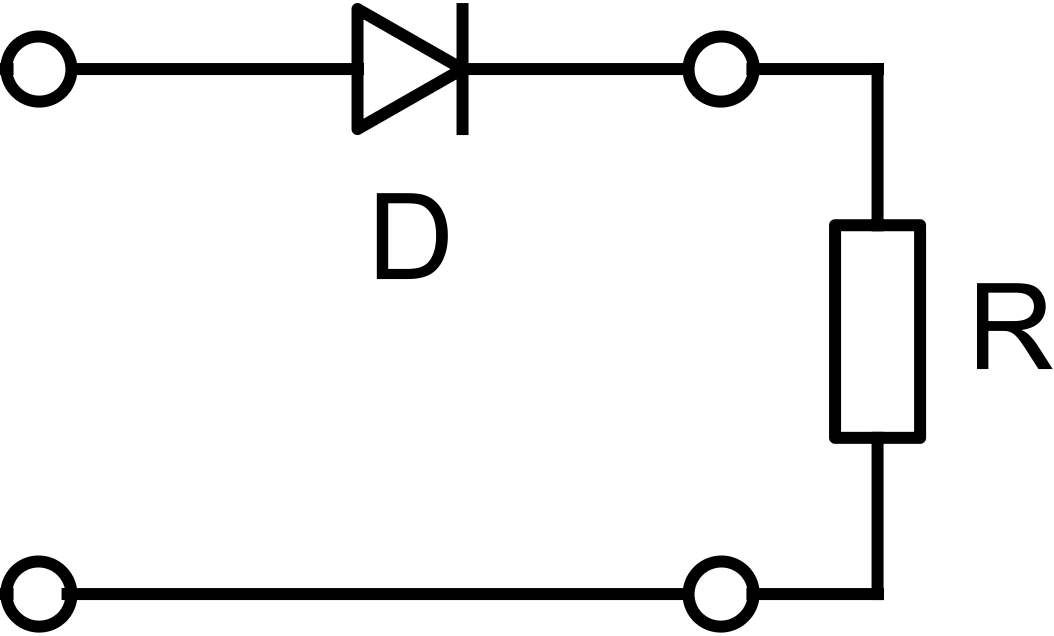
\includegraphics[width=0.2\textwidth]{half_wave_rectifier.png}
    \caption{will be replaced}
    \label{fig:hwr}
\end{figure}

A half-wave rectifier is less efficient than a full-wave rectifier, as it only uses one half of the AC cycle, leading to lower output voltage and higher ripple, requiring more filtering.

\begin{figure}[H]
    \centering
    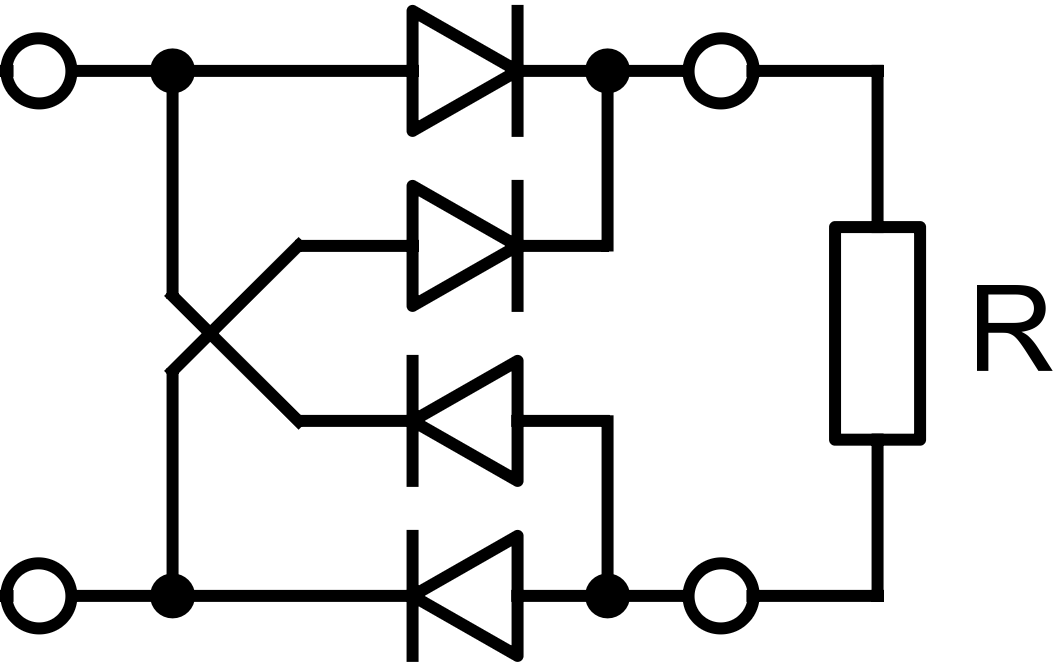
\includegraphics[width=0.2\textwidth]{full_wave_rectifier.png}
    \caption{will be replaced}
    \label{fig:fwr}
\end{figure}

In contrast, a full-wave rectifier makes use of both halves of the AC cycle, providing higher output efficiency and a smoother DC signal with less ripple.

The voltage drop in a diode occurs due to the energy required to overcome the potential barrier at the p-n junction. When forward-biased, electrons from the n-side need energy to cross the depletion region and recombine with holes, resulting in a forward voltage drop, typically around 0.7V for silicon diodes and 0.3V for germanium diodes. In this experiment, the voltage drop across diodes plays a crucial role in the rectification circuit. A full-wave rectifier using four diodes introduces a forward voltage drop that affects the overall output. When using LEDs as diodes, the forward voltage drop is higher, ranging from 1.8V to 3.3V, depending on the material and color. The objective is to evaluate how these voltage drops influence the effectiveness of the rectification process, particularly the amplitude and smoothness of the rectified DC output, which is critical for optimizing circuit efficiency and performance.

In a circuit composed solely of resistors and diodes, however, the voltage across the resistor does not stabilize due to the rapidly changing AC power supply. Therefore, to effectively convert the AC input into a steady DC output, additional circuit elements are required. When a capacitor  C  is connected in parallel with the resistor  R , the equation describing the circuit becomes as follows:

It is reasonable to assume the resistance of diode, denoted by $r$. In this experiment, various elements were used to check if it was converted into DC well. In particular, resistance, capacitor or diodes were used to verify  characteristics of the signal. If there are no elements, but just linked with cable, the output voltage is as follows.

\begin{equation}
    V_{NULL}  = V_0 \left|\sin(\omega t)\right|
\end{equation}

If the element is a resistance $R$, 

\begin{equation}
    V_R = \frac{R}{2r+R} V_0\left|\sin(\omega t)\right|
\end{equation}

If the element is a capacitor $C$,

\begin{equation}
    \frac{d}{dt}V_C + \frac{1}{RC}V_C = \frac{V_0}{RC}\left|\sin(\omega t)\right|
\end{equation}

While the absolute of sin function is as follows.
\[
    \left| \sin(x) \right|=\frac{2}{\pi} - \frac{4}{\pi} \sum_{k=1}^{\infty} \frac{\cos(2kx)}{4k^2-1} 
\]

Therefore,
\begin{equation}
    V_C = \frac{2}{\pi}V_0 - \frac{4}{\pi} \sum_{k=1}^{\infty} \frac{V_0}{4k^2-1} \mathrm{Re}(\frac {e^{2ik\omega t}}{2ik\omega RC+1})
\end{equation}


Figure ? illustrates the behavior of a capacitor discharging in a rectifier circuit and the resulting ripple voltage across the load. The voltage across the capacitor decays exponentially as it discharges through the load, following the equation: (would modify soon)

\[
V = V_{p(in)} e^{-t/RC}
\]

where \( V_{p(in)} \) is the peak input voltage, \( t \) is the time, and \( RC \) is the time constant of the circuit. The peak-to-peak ripple voltage, \( V_r(pp) \), can be approximated as:
\[
V_r(pp) = \frac{V_{p(in)}}{2f RC}
\]
This equation indicates that the ripple voltage decreases with larger values of \( RC \), showing the importance of the time constant in minimizing ripple.
The RMS value of the ripple voltage for this sawtooth-like waveform is given by:
\[
V_r(rms) = \frac{V_{p(in)}}{4\sqrt{3}f RC}
\]
Additionally, the DC component \( V_{dc} \) is impacted by the ripple voltage, and for small ripple conditions, \( t_{dis} \approx T \), where \( T \) is the period of the AC input. The DC voltage is calculated as:

\[
V_{dc} = V_{p(in)} \left( 1 - \frac{1}{4f RC} \right)
\]

This relationship shows how the average DC voltage is slightly reduced due to the ripple effect. The analysis is essential for understanding the capacitor's smoothing role in rectification and how the choice of \( RC \) values influences output quality.


\section{Experiment}
\subsection{Apparatus}
The rectification circuit is constructed by four diodes, working in AC voltage provided by Analog Discovery 2 (\cite{digilent_analog_discovery}).
The frequency is varied from $0.02 \mathrm{Hz}$ to $200 \mathrm{Hz}$ in logarithmic scale, at 40 sampling points.
For each frequency experiment, the output voltage of exactly ten period of each drive voltage is measured.
We wanted to modify the capacitance of the circuit, used 4 $4.7 \mu \mathrm{F}$ and 1 $100 \mu \mathrm{F}$ capacity capacitor.
The serially connected capacitor is examined, five different situation is tested.
True capacitance value of each component is measured by multimeter, and its result is presented at Fig. \ref{table: capacity data}.
By the true value measured, the circuit capacity of $90.86 \mu \mathrm{F}$, $4.622 \mu \mathrm{F}$, $2.255 \mu \mathrm{F}$, $1.478 \mu \mathrm{F}$, and $1.115 \mu \mathrm{F}$ be the circuit capacity condition of each experiments.

\begin{figure}[H]
    \centering
    \begin{tabular}{c|c}
        \textbf{Index} & \textbf{Measured Capacitance} \\ 
        \hline
        \hline
        4.7 \#1 & $4.622 \pm 0.002 \mu \mathrm{F}$ \\ 
        \hline
        4.7 \#2 & $4.405 \pm 0.002 \mu \mathrm{F}$ \\
        \hline
        4.7 \#3 & $4.288 \pm 0.002 \mu \mathrm{F}$ \\
        \hline
        4.7 \#4 & $4.543 \pm 0.002 \mu \mathrm{F}$ \\
        \hline
        100 \#1 & $90.86 \pm 0.02 \mu \mathrm{F}$ \\
        \hline
    \end{tabular}
    \caption{
        The measured capacitance of each capacitor component.
        The index is labeled by the factory value denoted in arbitrary order.
    }
    \label{table: capacity data}
\end{figure}

\subsection{Methods}
 Construct the circuit as (figure), and plug drive voltage to the input node respectively.
 Connect the nodes between drive voltage in Channel 1, and output voltage in Channel 2 of Analog Discovery 2 Oscilloscope.
 Turn on the sinosodic signal of $2.5V$ and modified frequency in order to the drive voltage, and wait for 1 second for the circuit to be saturated.
 Measure $100$ points per period for sampling, for 10 period duration.
 Grab the initial time data and construct time grid for each measured result.

 The machine works by the python code built, with SDK provided by \cite{digilent_analog_discovery}.
 The code for such frequency sweep experiment is denoted in \ref{Appendix: Codes}.

\section{Results and Conclusion}
 The term drive voltage denotes the total voltage applied to the circuit, before rectified.
 And, the term reaction voltage means the measured voltage after rectified across capacitor.
 The performance of the DC filter can be measured by the difference of the max and min value of the reaction produced, conventionally called as ripple voltage.
 The diode and the rest of the circuit capacitance is about few $\mathrm{pF}$, so that is totally negliable from the external capacity attatched.
 
\begin{figure}[H]
    \begin{subfigure}[b]{8cm}
        \centering
        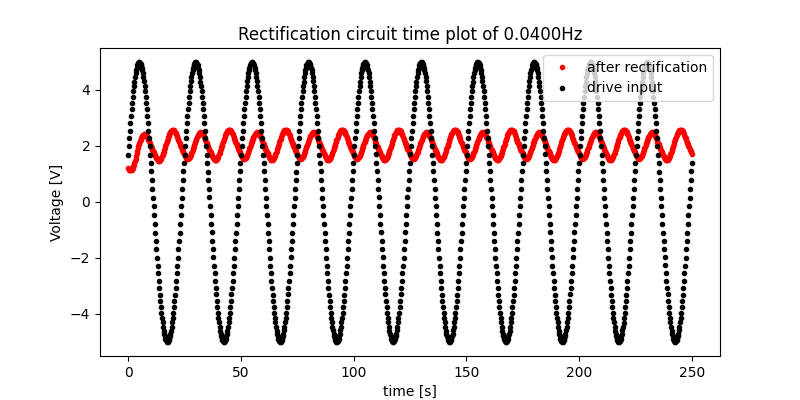
\includegraphics[width=8cm]{../../../rectification_results/raw_figs(4.7uF)/drive_frequency (0.0400).png}
        \caption{}
    \end{subfigure}
    \hfill
    \begin{subfigure}[b]{8cm}
      \centering
      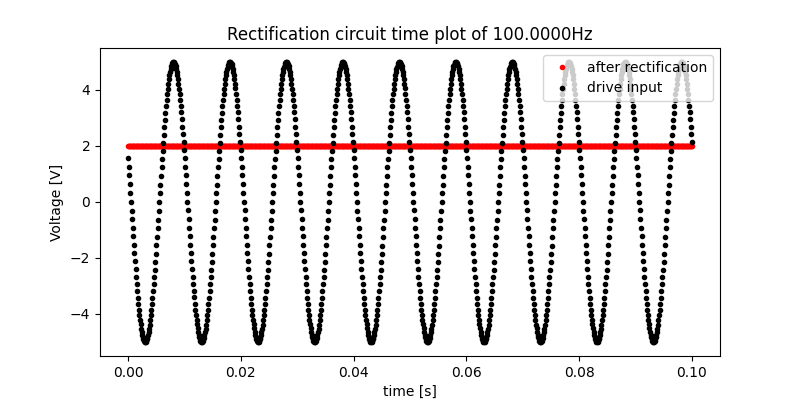
\includegraphics[width=8cm]{../../../rectification_results/raw_figs(4.7uF)/drive_frequency (100.0000).png}
      \caption{}
  \end{subfigure}
  \hfill
  \centering
  \hfill
    \caption{
        The Voltage [V] - time [s] plot of the ripple circuit.
        4.7 \#1 capacitor is used for both result.
        (a) in drive frequency $0.04 \mathrm{Hz}$.
        (b) in drive frequency $100.0 \mathrm{Hz}$.
        The output signal is almost DC for high frequency, where the low frequency signal have ripple voltage.
    }
    \label{fig: example figure}
\end{figure}

Fig. \ref{fig: example figure} shows the time series raw data of reaction and the drive voltage of capaciy $4.6 \mathrm{\mu F}$.
Fig. \ref{fig: example figure} (a) is the data of drive frequency $0.04 \mathrm{Hz}$, and (b) is for the drive frequency $100.0 \mathrm{Hz}$
As expected, the ripple voltage value gets lower when the frequency gets higher.
There are asymmetry found for half period rectification, the reason for the error is discussed below (!ref todo)

\begin{figure}[H]
    \begin{subfigure}[b]{6cm}
        \centering
        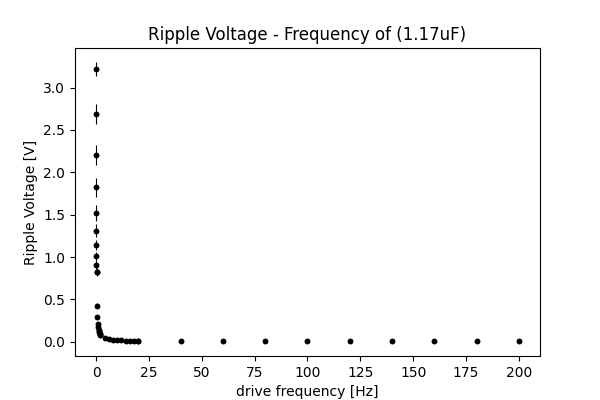
\includegraphics[width=6cm]{../../../rectification_results/ripple_voltage_frequency_(1.17uF)_(20).png}
        \caption{}
    \end{subfigure}
    \hfill
    \begin{subfigure}[b]{6cm}
      \centering
      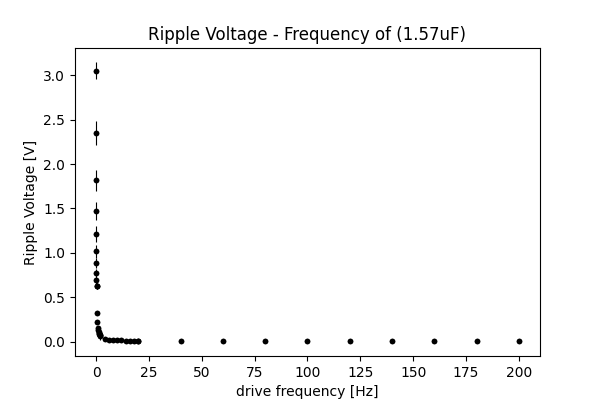
\includegraphics[width=6cm]{../../../rectification_results/ripple_voltage_frequency_(1.57uF)_(20).png}
      \caption{}
  \end{subfigure}
  \centering
  \hfill
    \caption{
        The ripple voltage to the drive frequency of two different circuit capacitance.
        (a) $1.17 \mathrm{\mu F}$, (b) $1.57 \mathrm{\mu F}$.
        The error bar is calculated by the peak height differ from each period.
        The figure of different kind of capacitance is provided in \ref{fig: log V-log f figure Supplementary}.
    }
    \label{fig: V-f figure}
\end{figure}

To observe the exact dependancy of the ripple voltage by the driving frequency, the plot of each capacitance required.
Fig. \ref{fig: V-f figure}, for some results and the \ref{fig: V-f figure Supplementary} shows the direct plot of ripple voltage and the drive frequency in various kinds of capacitance value.
The ripple voltage is almost 0 at high frequency, and increase fast near low frequency area, and peaks high over the working amplitude.
The theory predicts the relation of the ripple voltage and the drive frequency as approximally $V_{\mathrm{rip}} = \frac{I}{f C}$.
For the extremely low or high frequency, the approximation fails, the results should be considered as complex differential equation.
We simulated the results, and denoted on (ref! todo)

In the well performing area, the linear regresssion is applied for $\mathrm{log} V- \mathrm{log} f$ plot and its statics shown below.

\begin{figure}[H]
    \begin{subfigure}[b]{6cm}
        \centering
        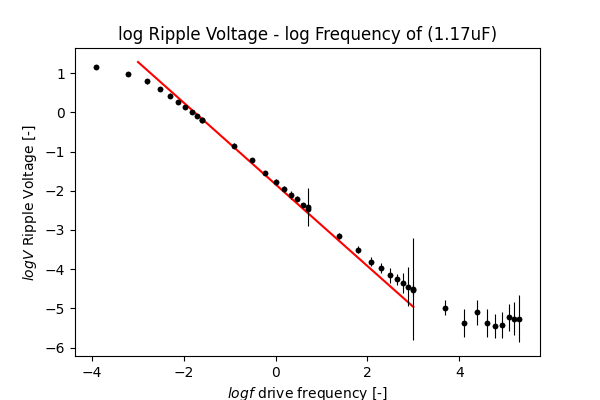
\includegraphics[width=6cm]{../../../rectification_results/ripple_voltage_frequency_log_log_(1.17uF)_20.png}
        \caption{}
    \end{subfigure}
    \hfill
    \begin{subfigure}[b]{6cm}
      \centering
      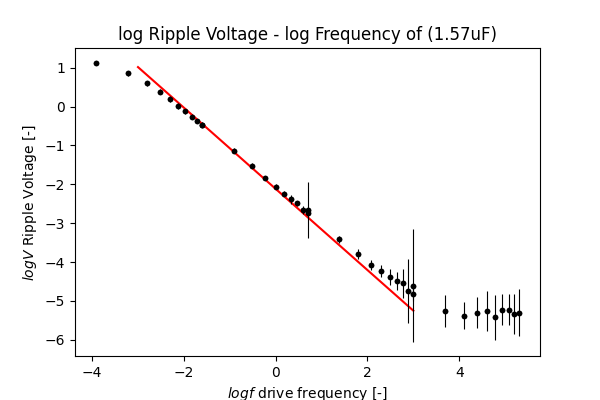
\includegraphics[width=6cm]{../../../rectification_results/ripple_voltage_frequency_log_log_(1.57uF)_20.png}
      \caption{}
  \end{subfigure}
  \centering
  \hfill
    \caption{
        The ripple voltage to the drive frequency of two different circuit capacitance in logarithmic scale is plotted.
        The linear regression of the well performing area is also depicted.
        (a) $1.17 \mathrm{\mu F}$, (b) $1.57 \mathrm{\mu F}$.
        The error bar is calculated by the peak height differ from each period.
        The figure of different kind of capacitance is provided in \ref{fig: V-f figure Supplementary}.
    }
    \label{fig: log V-log f figure}
\end{figure}


\begin{figure}[H]
    \centering
    \begin{tabular}{c|c|c|c}
        \textbf{C} & \textbf{a} & \textbf{b} & $\mathrm{R^2}$ \\ 
        \hline
        \hline
        $1.17uF$ & $-1.04\pm0.01$ & $-1.84\pm0.01$ & $1.000$  \\
        \hline
        $1.57uF$ & $-1.04\pm0.01$ & $-2.11\pm0.01$ & $0.999$  \\
        \hline
        $2.35uF$ & $-1.05\pm0.01$ & $-2.53\pm0.01$ & $0.999$  \\
        \hline
        $4.7uF$ & $-1.089\pm0.02$ & $-3.30\pm0.02$ & $0.994$  \\
        \hline
        $100uF$ & $-2.16\pm0.21$ & $-10.85\pm0.21$ & $0.828$  \\
        \hline
    \end{tabular}
    \caption{
        The measured capacitance of each capacitor component.
        The index is labeled by the factory value denoted in arbitrary order.
    }
    \label{table: linear regression of log log plot}
\end{figure}


\section{References}
\bibliographystyle{plain} 
\bibliography{recref}
\end{multicols}
\newpage

\section{Appendix}
\subsection{Codes for AD2}
\label{Appendix: Codes}
The code and relavent wrapper library is open to public in \cite{github}.
\begin{lstlisting}[language=Python, caption={Python Code Example}]
from pydwf import DwfLibrary
from pydwf.utilities import openDwfDevice
import numpy as np
from libs.pydwf_wrapper import generate_sine_wave, measure_voltage
import matplotlib.pyplot as plt
import time
from alive_progress import alive_bar

dwf = DwfLibrary()
def experiment(experiment_config):
    create_folder(results_folder)
    with openDwfDevice(dwf) as device:
        total_results = []
        amplitude = 5
        freq_ini = 0.02
        freq_fin = 0.2
        num = 10

        with alive_bar(num) as bar:
            for frequency in np.linspace(freq_ini, freq_fin, num):

                output_channel = device.analogOut
                generate_sine_wave(
                    output_channel, frequency=frequency, amplitude=amplitude
                )

                time.sleep(1)
                input_channel = device.analogIn
                result = measure_voltage(
                    input_channel,
                    record_time=1 / frequency * 10,
                    sampling_frequency=frequency * 100,
                    number_of_channel=2,
                )

                config_dict = experiment_config.copy()
                config_dict["frequency"] = frequency
                config_dict["amplitude"] = amplitude
                result["config"] = config_dict

                total_results.append(result)
                bar()

    return total_results
\end{lstlisting}

\subsection{Supplementary}

\begin{figure}[H]
  \begin{subfigure}[b]{5cm}
    \centering
    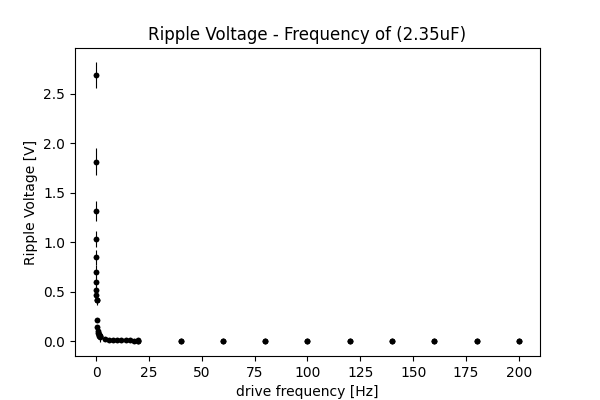
\includegraphics[width=5cm]{../../../rectification_results/ripple_voltage_frequency_(2.35uF)_(20).png}
    \caption{}
\end{subfigure}
\begin{subfigure}[b]{5cm}
    \centering
    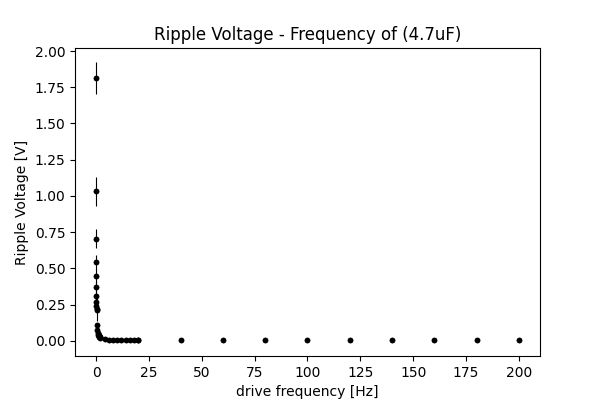
\includegraphics[width=5cm]{../../../rectification_results/ripple_voltage_frequency_(4.7uF)_(20).png}
    \caption{}
\end{subfigure}
\begin{subfigure}[b]{5cm}
    \centering
    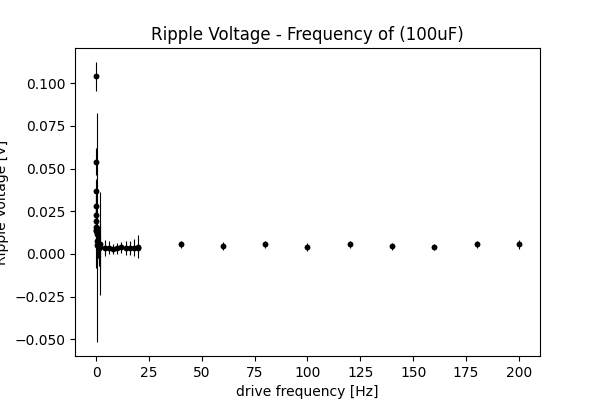
\includegraphics[width=5cm]{../../../rectification_results/ripple_voltage_frequency_(100uF)_(20).png}
    \caption{}
\end{subfigure}
  \hfill
  \centering
  \hfill
    \caption{
        The ripple voltage to the drive frequency of two different circuit capacitance.
        (a) $2.35 \mathrm{\mu F}$, (b) $4.7 \mathrm{\mu F}$, (c) $100 \mathrm{\mu F}$.
        The error bar is calculated by the peak height differ from each period.
        This is the supplementary figure of \ref{fig: V-f figure}.
    }
    \label{fig: V-f figure Supplementary}
\end{figure}

\begin{figure}[H]
    \begin{subfigure}[b]{5cm}
        \centering
        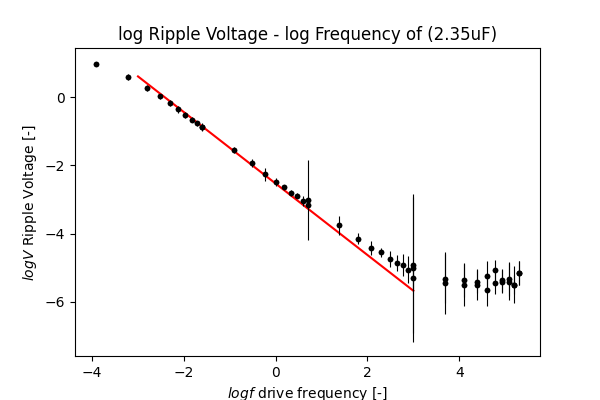
\includegraphics[width=5cm]{../../../rectification_results/ripple_voltage_frequency_log_log_(2.35uF)_20.png}
        \caption{}
    \end{subfigure}
    \hfill
    \begin{subfigure}[b]{5cm}
      \centering
      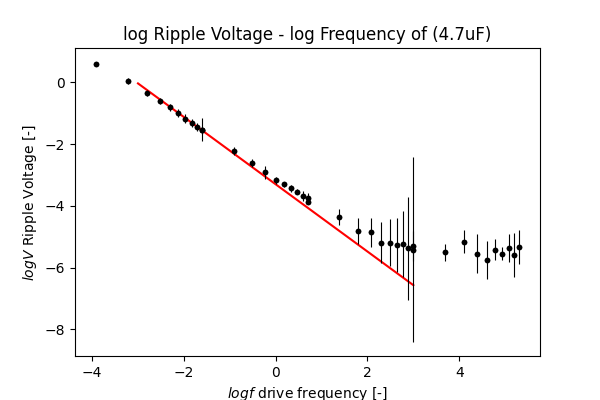
\includegraphics[width=5cm]{../../../rectification_results/ripple_voltage_frequency_log_log_(4.7uF)_20.png}
      \caption{}
  \end{subfigure}
  \hfill
  \centering
  \hfill
    \caption{
        The ripple voltage to the drive frequency of two different circuit capacitance in logarithmic scale is plotted.
        The linear regression of the well performing area is also depicted.
        (a) $2.35 \mathrm{\mu F}$, (b) $4.7 \mathrm{\mu F}$.
        The error bar is calculated by the peak height differ from each period.
        The figure of different kind of capacitance is provided in \ref{fig: log V-log f figure}.
    }
    \label{fig: log V-log f figure Supplementary}
\end{figure}
\end{document}